\documentclass{ieeetmlcn}
\usepackage{cite}
\usepackage{amsmath,amssymb,amsfonts}
\usepackage{algorithmic}
\usepackage{graphicx,color}
\graphicspath{{figures/}}
\usepackage{textcomp}
\usepackage{xcolor}
\usepackage{booktabs}
\usepackage{hyperref}
\hypersetup{hidelinks=true}
\usepackage{algorithm,algorithmic}
\def\BibTeX{{\rm B\kern-.05em{\sc i\kern-.025em b}\kern-.08em
    T\kern-.1667em\lower.7ex\hbox{E}\kern-.125emX}}
\AtBeginDocument{\definecolor{tmlcncolor}{cmyk}{0.93,0.59,0.15,0.02}\definecolor{NavyBlue}{RGB}{0,86,125}}




\def\OJlogo{\vspace{-4pt}
\includegraphics[height=18pt]{new_logo}}
\def\seclogo{\vspace{10pt}
\includegraphics[height=18pt]{new_logo}}

\def\authorrefmark#1{\ensuremath{^{\textbf{#1}}}}

\begin{document}
\receiveddate{XX Month, XXXX}
\reviseddate{XX Month, XXXX}
\accepteddate{XX Month, XXXX}
\publisheddate{XX Month, XXXX}
\currentdate{XX Month, XXXX}
\doiinfo{TMLCN.2022.1234567}
\jvol{--}
\pubyear{2026}

\markboth{}{Grau Garcia \textit{et al.}: Risk-Aware Distributional Reinforcement Learning for 5G-Advanced Handover Decisions}

\title{Risk-Aware Distributional Reinforcement Learning for 5G-Advanced Handover Decisions}

\author{Gerard Grau Garcia, Ainna Yue Moreno-Locubiche,\\ Josep Vidal, Senior Member IEEE, Margarita Cabrera-Bean, Senior Member IEEE}
\affil{\textit{Dept. of Signal Theory and Communications, Universitat Politècnica de Catalunya - BarcelonaTech (UPC), 08034, Spain}}
\corresp{Corresponding author: Gerard Grau Garcia (email: gerard.grau.garcia@estudiantat.upc.edu).}
\authornote{This work covers activities of the project 6-SENSES grant PID2022-138648OB-I00, supported by MCIN/AEI/10.13039/501100011033, and by ERDF-EU.}


\begin{abstract}
Lower-layer triggered mobility (LTM) in 5G-Advanced accelerates cell switches by executing pre-configured handovers via Layer 1 / Layer 2 (L1/L2) channel measurements, substantially reducing user-plane interruption time. However, making fast handover decisions under rapid multipath channel fading poses severe reliability risks, where suboptimal decisions lead to costly handover failures (HOF) and radio link failures (RLF). While standard deep reinforcement learning (RL) such as Deep Q-Networks (DQN) achieves higher spectral efficiency and greater signaling frugality than legacy 3GPP heuristics, we uncover a critical \emph{out-of-domain generalization gap}: scalar DQN fits the local channel profiles of the training trajectories and suffers an almost two-fold increase in failure rate (from $0.67$ to $1.12$\,HOF/min) when evaluated on unseen channel fading realizations. To overcome this fundamental limitation, we propose a risk-aware distributional reinforcement learning framework based on Quantile Regression DQN (QR-DQN). We show that learning the full return distribution across $N=25$ quantiles acts as a powerful regularizer, restoring out-of-domain generalization. Furthermore, we reveal that while naive tail truncation (training only on the worst-case quantiles) suffers from severe tail-overfitting and gradient starvation, a smooth two-step distortion (\emph{Soft-step}, $\alpha=0.25, r=2.0$) safely guides actions toward risk aversion while preserving full distributional training. Evaluated across 1,000 completely unseen mobile user trajectories over 5 independent seeds, Soft-step achieves the lowest failure rate in the benchmark ($0.74$ HOF/min), halves control-plane signaling overhead compared to 3GPP heuristics ($5.8$ vs. $11.3$ handovers/min), and preserves full spectral efficiency ($4.04$ bps/Hz), avoiding the 7\% throughput penalty incurred by contextual bandits.
\end{abstract}

\begin{IEEEkeywords}
5G-Advanced, lower-layer triggered mobility, distributional reinforcement learning, quantile regression, out-of-domain generalization, risk-sensitive control, conditional value at risk.
\end{IEEEkeywords}

\maketitle

\section{Introduction}

Fifth-generation (5G) and 5G-Advanced radio access networks deploy dense, multi-sector cellular topologies operating at higher frequency bands. As user equipments (UEs) move through these dense networks, they cross cell and sector boundaries frequently, necessitating rapid and reliable mobility management. Each handover (HO) is a high-stakes reconfiguration: executed properly, it sustains peak spectral efficiency and guarantees continuous connectivity; executed poorly or tardily, it triggers handover failures (HOF), radio link failures (RLF), or wasteful ``ping-pong'' (PP) oscillations back to the previously serving cell.

To address the latency limitations of legacy Radio Resource Control (RRC) signaling, 3GPP Release 18 introduced \emph{Lower-Layer Triggered Mobility} (LTM)~\cite{eric2024}. LTM decouples candidate cell preparation from execution by pre-configuring candidate target cells at higher layers and executing the cell switch dynamically via fast Medium Access Control (MAC) control elements (CE) driven by Layer 1 / Layer 2 (L1/L2) channel measurements. While LTM minimizes interruption time, it shifts the operational challenge to making cell selection decisions under fast-fading channel variations without the smoothing benefit of slow Layer 3 filtering. That selection is the decision problem we study.

Prior learning-based approaches have cast cell selection as heuristic rules, contextual multi-armed bandits (CMAB), or surveyed various reinforcement learning formulations for handover optimization~\cite{alraih2022}. While myopic bandit formulations improve safety compared to rigid 3GPP thresholds, their one-step objective ($\gamma = 0$) optimizes only immediate channel gains, rendering them unable to anticipate future signal degradation and causing a notable throughput capacity penalty. Conversely, standard Reinforcement Learning (RL) techniques like Deep Q-Networks (DQN)~\cite{dqn} optimize long-term discounted rewards ($\gamma = 0.9$). However, scalar DQN learns only the expected return $\mathbb{E}[R]$, which fails to account for the dispersion and extreme tail risks inherent to wireless fading channels.

Crucially, in this paper we uncover a major vulnerability in applying standard deep RL to wireless mobility: the \textbf{Out-of-Domain Generalization Gap}. When scalar DQN is trained and tested on the same channel realizations, it appears to perform well. Yet, when evaluated on completely unseen mobility trajectories, its handover failure rate nearly doubles. Scalar value learners overfit to local fading variations rather than discovering generalizable transition dynamics.

To solve this challenge, we introduce a risk-aware distributional reinforcement learning framework:
\begin{itemize}
  \item We formulate 5G LTM handover as a Markov Decision Process (MDP) and implement a rigorous out-of-domain evaluation protocol, training on 2,000 UEs and validating greedily on 1,000 disjoint, unseen test trajectories.
  \item We demonstrate that modeling the full return distribution using Quantile Regression DQN (QR-DQN)~\cite{qrdqn} provides a rich training signal that acts as an implicit regularizer, completely closing the scalar generalization gap.
  \item We investigate risk-aware policies and expose the pitfall of \emph{Truncated Risk} (learning only the tail), which leads to policy instability and tail-overfitting. Similarly, strict Conditional Value at Risk (Hard CVaR) induces a ``policy paralysis'' trap where the agent over-reserves resources but hesitates to switch cells.
  \item We propose \textbf{Soft-step QR-DQN}, a spectral risk formulation where $\alpha \in (0, 1]$ parameterizes the lower tail fraction (risk level) and $r \ge 1$ governs the smooth tail distortion ratio. While training on the complete return distribution, this smoothly upweights the lower tail during decision-making. Across 9 standardized KPIs over 5 independent seeds, Soft-step achieves the lowest failure rate in the benchmark ($0.74$ HOF/min) and preserves peak capacity ($4.04$ bps/Hz) without the 7\% capacity penalty of contextual bandits.
\end{itemize}


% =====================================================================
\section{Background and Related Work}
\label{sec:related}

\subsection{LTM and Handover Optimization}
In legacy mobility the network reconfigures a UE's serving cell through
higher-layer (RRC) signaling driven by filtered network-protocol L3 measurements---robust but slow~\cite{eric2024}.
\emph{Lower-layer triggered mobility} (LTM) instead prepares one or more candidate cells in advance and lets a fast L1/L2 measurement event trigger the execution of a pre-configured switch, reducing the interruption time but tightening the decision loop.
The operational cost of a mobility policy is captured by a small set of events: a \emph{handover} (HO) whenever the serving cell changes, a \emph{ping-pong} (PP) when the UE returns to a recently left cell within a short window, a \emph{handover failure} (HOF) when the target
link cannot be established, and a \emph{radio-link failure} (RLF) when the serving link collapses after a sustained run of out-of-sync observations within a time window.
A good policy minimizes HOF and PP while sustaining spectral efficiency.

Prior learning-based work optimizes this trade-off with heuristics over an expected-KPI objective. The work in \cite{cmab_ho} optimizes network decisions by maximizing an expected objective using contextual bandits. To further enhance signal quality and target pre-selection, this framework is optionally augmented with Reconfigurable Intelligent Surfaces (RIS) and LMMSE channel prediction, showcasing how physical-layer enhancements can be stacked on top of decision-making layers to stabilize vehicular or cellular links. While this represents the closest baseline to our work, it remains strictly risk-neutral. Our proposed framework directly addresses this limitation by introducing risk-awareness into the decision-making process.


\subsection{Distributional Reinforcement Learning}
\label{sec:rel-distrl}
Distributional RL predicts the full distribution of the return rather than its expectation. Instead of modeling the scalar action-value $Q(x,a)$ for each state $x$ and action $a$, the agent models the return as a random variable $Z(x,a)$ that obeys the distributional Bellman equation:
\begin{equation}
Z(x,a) \overset{D}{=} R(x,a) + \gamma\,Z(X',A'),
\label{eq:dist-bellman}
\end{equation}
where $\overset{D}{=}$ denotes equality in distribution, $R(x,a)$ is the reward, $\gamma$ the discount factor, and $(X',A')$ the (random) next state--action pair.
Even when the policy ultimately acts on the mean $\mathbb{E}[Z(x,a)]$, learning the distribution provides a richer per-update signal and consistently improves the resulting policy.
Most practical distributional RL algorithms approximate the cumulative distribution as a staircase function; representative methods include C51~\cite{c51}, QR-DQN~\cite{qrdqn}, IQN~\cite{iqn} and FQF~\cite{fqf}.
We build on QR-DQN, which parametrizes the distribution by estimating the locations of a fixed set of quantiles. Unlike Implicit Quantile Networks (IQN)~\cite{iqn} or Fully Parameterized Quantile Function (FQF)~\cite{fqf}, which introduce auxiliary quantile proposal networks and require run-time stochastic sampling, QR-DQN operates on a fixed, deterministic set of quantiles. This yields a closed-form quantile Huber loss and deterministic inference with minimal computational latency and footprint, a critical requirement for high-cadence 5G L1/L2 LTM decision loops.


\subsection{Risk-Sensitive Reinforcement Learning}
\label{sec:rel-risk}
In standard distributional RL the greedy action maximizes the expected return $\mathbb{E}[Z(x,a)]$. In vanilla QR-DQN with midpoint quantiles, this expectation is approximated by the uniform average of the $N$ predicted quantiles $\tfrac{1}{N}\sum_{i=1}^{N}\theta_i(x,a)$, which represents the risk-neutral special case with uniform weights $w_i = 1/N$. Intuitively, each quantile $\theta_i(x, a)$ specifies the exact position on the horizontal axis of the return distribution corresponding to a fixed probability checkpoint when action $a$ is executed at state $x$. One may instead aggregate the $\theta_i$ under a different weighting criterion to obtain a risk-sensitive policy. Selecting an action from a set of competing return distributions is fundamentally non-trivial because distributions lack a canonical total order---under stochastic dominance, many pairs are incomparable. Any scalar aggregation must therefore impose an explicit ordering, directly encoding a specific risk attitude.

A common risk-averse choice replaces the expectation with the Conditional Value at Risk at level $\alpha$, $\mathrm{CVaR}_\alpha$, defined as the average of the worst $\alpha$-fraction of outcomes. Here $\alpha \in (0, 1]$ is the tail fraction that is integrated, not an individual quantile position. More generally, replacing the uniform average by non-negative quantile weights $\sum_{i=1}^N \omega_i \theta_i(x,a)$ with $\sum_i \omega_i = 1$ yields a \emph{spectral} (or distortion) risk measure~\cite{acerbi}, with the risk-neutral expectation ($\omega_i = 1/N$) and $\mathrm{CVaR}_\alpha$ ($\omega_i = \mathbb{I}\{i \le k\}/k$) as specific piecewise-uniform instances. This weighted-quantile framework defines the design space for the risk-aware policies we study.

CVaR and related risk-sensitive criteria have a rich history in optimization and control: Rockafellar and Uryasev~\cite{rockafellar} established convex optimization techniques for CVaR; Chow and Ghavamzadeh~\cite{chow2014} formulated CVaR objectives for Markov Decision Processes; and Tamar \textit{et al.}~\cite{tamar2015} developed policy gradient methods for risk-averse evaluation. Distributional RL makes evaluating such criteria particularly straightforward and computationally direct, since the return quantiles needed to compute $\mathrm{CVaR}_\alpha$ and spectral measures are predicted explicitly by the neural network without requiring secondary sampling loops.

\subsection{Distributional RL in Wireless Communications}
\label{sec:rel-wireless}
While the initial successes of distributional RL focused primarily on arcade games, autonomous driving, and robotics, recent literature has successfully deployed distributional frameworks to address optimization challenges within next-generation wireless networks. In~\cite{EldeebConservative}, the Conservative Q-Learning (CQL) algorithm introduces a regularization term to the DQN objective function to address overestimation bias in offline learning by penalizing discrepancies between estimated returns across all actions and the values recorded in the dataset. In~\cite{EldeebOffline}, CQL is combined with Quantile Regression (QR-DQN) for unmanned aerial vehicle (UAV) trajectory optimization. In~\cite{Liu24}, quantile regression deep Q-networks are deployed to learn the complete cumulative distribution of end-to-end delays rather than simple averages, optimizing routing decisions under deadline constraints and preventing traffic bottlenecks.

To the best of our knowledge, our work is the first to investigate risk-aware distributional RL for 5G-Advanced lower-layer mobility decisions. Furthermore, in contrast to prior art, this paper focuses on out-of-domain generalization across fading profiles and the downstream distortion of predicted quantiles to prevent tail failures.

\section{System Model and Problem Formulation}
\label{sec:model}

\subsection{5G LTM Deployment and Simulator}
We consider a cellular deployment of $N_{\text{BS}} = 7$ tri-sector base stations ($21$ sectors) serving mobile UEs moving along urban trajectories at vehicular speeds. Channel gains between sectors and UEs incorporate distance-dependent path loss, shadow fading, and small-scale multipath fast fading generated from calibrated ray-tracing and geometric models. The simulator advances at a $10$\,ms tick resolution: at each step it derives the serving signal-to-interference-plus-noise ratio (SINR) from channel gains, transmit power ($P_{\text{tx}} = 25$\,dBm), and inter-cell interference, mapping it through a modulation-and-coding scheme (MCS) to spectral efficiency. An SINR below the outage threshold ($-3$\,dB) yields zero bit rate, and a sustained run of out-of-sync indications escalates to a radio-link failure (RLF). System parameters (Table~\ref{tab:sysparams}) follow the calibrated LTM reference implementation of~\cite{cmab_ho}.

LTM maintains a small set of \emph{prepared} candidate cells (up to $N_{\text{prep}}^{\max} = 5$), selected from the strongest neighbors by an RSRP threshold ($\Delta_{\text{prep}} = -3$\,dB). In the standard heuristic, a prepared cell is executed when its RSRP exceeds the serving cell by an execution margin ($H_{\text{exec}} = 3$\,dB). We replace this rigid execution trigger with our learned agent: at each decision step, the agent chooses whether to stay or execute an LTM switch to a prepared cell.

\subsection{Rigorous Out-of-Domain Generalization Split}
\label{sec:data-split}
Unlike prior studies that train and evaluate on the same channel realizations, we enforce a strict separation between training and evaluation:
\begin{itemize}
    \item \textbf{Training Set:} 2,000 independent mobility trajectories, trained across 6,000 episodes (ensuring 3 full passes per trajectory).
    \item \textbf{Test Set:} 1,000 completely separate, unseen trajectories, evaluated greedily ($\epsilon = 0.0$) across 5 random seeds to measure true out-of-domain generalization.
\end{itemize}

\begin{table}[htbp]
\caption{Calibrated System and Simulation Parameters}
\label{tab:sysparams}
\centering
\begin{tabular}{|l|c|}
\hline
\textbf{Parameter} & \textbf{Value} \\
\hline
Base stations $\times$ sectors      & $7 \times 3 = 21$ \\
Training trajectories               & $2{,}000$ ($300$\,s each) \\
Evaluation trajectories (unseen)    & $1{,}000$ ($300$\,s each) \\
Simulator step / RL cadence         & $10$\,ms / $100$\,ms event-driven \\
Transmit power ($P_{\text{tx}}$)   & $25$\,dBm \\
Thermal noise floor ($\sigma^2$)    & $-101$\,dBm ($20$\,MHz bandwidth) \\
Receiver sensitivity threshold      & $-95$\,dBm \\
Outage (RLF) SINR threshold         & $-3$\,dB \\
Preparation offset ($\Delta_{\text{prep}}$) & $-3$\,dB \\
Max.\ prepared candidate cells      & $5$ \\
Execution offset (LTM trigger)$^{\dagger}$ & $3.0$\,dB \\
Execution time ($T_{\text{exec}}$)  & $40$\,ms \\
\hline
\end{tabular}
{\footnotesize $^{\dagger}$The $+3$\,dB execution offset is the LTM baseline's
hard handover trigger; the RL agent replaces it with a learned, value-based
decision.}
\end{table}

\subsection{MDP Formulation}
\label{sec:mdp}
We model LTM HO as a Markov decision process in which the agent acts only at
handover-decision opportunities. These arise once per LTM cycle and are
unevenly spaced in time; we index the agent's successive decisions by $t$ and
treat each as one step.

\textbf{State.} An $88$-dimensional vector: UE speed $(1)$ and serving-cell
tenure $(1)$, the one-hot serving sector $(21)$, per-sector RSRP $(21)$,
moving-average MCS $(21)$ and moving-average SINR $(21)$, and the UE position
$(x,y)$ $(2)$.

\textbf{Action.} At each decision the agent chooses a target from the action set
$\{\text{serving}\}\cup\{\text{prepared}\}$, at most six entries, since
preparation caps the candidate list at $5$. Choosing the serving cell is a
\emph{stay} (no handover); choosing a non-serving prepared cell executes a
handover to it. Because the agent itself fires the handover, it replaces LTM's
$+3$\,dB execution trigger with the learned value of acting now versus staying,
while preparation and the candidate restriction remain the reference heuristic methodology of \cite{eric2024}.

\textbf{Reward.} Each decision is rewarded over the interval until the next
decision by the multiplicative LTM HO reward of~\cite{cmab_ho},
\begin{equation}
R_t = R^{\mathrm{thr}}_t \,\cdot\,
      \frac{\alpha_{\mathrm{HO}}^{\,\mathbb{I}^{\mathrm{HO}}_t}\;
            \alpha_{\mathrm{PP}}^{\,\mathbb{I}^{\mathrm{PP}}_t}\;
            \alpha_{\mathrm{HOF}}^{\,\mathbb{I}^{\mathrm{HOF}}_t}}
           {1 + e^{\,2\,(N^{\mathrm{OOS}}_t - 2)}},
\label{eq:reward}
\end{equation}
where $R^{\mathrm{thr}}_t$ is the throughput term---the serving spectral
efficiency (bps/Hz) \emph{averaged over the decision interval}; the indicators
$\mathbb{I}^{\mathrm{HO}}_t,\mathbb{I}^{\mathrm{PP}}_t,\mathbb{I}^{\mathrm{HOF}}_t\in\{0,1\}$
flag whether a handover, ping-pong or handover failure occurred \emph{anywhere
within} that interval; and
$\alpha_{\mathrm{HO}},\alpha_{\mathrm{PP}},\alpha_{\mathrm{HOF}}\in(0,1]$ are the
corresponding multiplicative penalties (defaults $\alpha_{\mathrm{HOF}}{=}0.1$,
$\alpha_{\mathrm{HO}}{=}0.8$, $\alpha_{\mathrm{PP}}{=}0.9$, so a failure is
penalized far more harshly than a routine handover). The final factor is a
reverse sigmoid of the out-of-sync counter $N^{\mathrm{OOS}}_t$ (the number of
consecutive out-of-sync indications on the serving link): it stays near $1$
while the link is in sync, equals $0.5$ at $N^{\mathrm{OOS}}_t{=}2$, and decays
toward $0$ as the link approaches radio-link failure.
As the penalty factors lie in $(0,1]$, the reward formulation discounts the ideal throughput $R^{\mathrm{thr}}_t$ according to the penalties triggered by mobility failures and link degradation, which the distributional agent models as a random
return.

Because decisions are event-driven, a policy's own choices change how many actions it
faces per episode; we therefore compare policies by their mean reward
\emph{per decision} rather than the episode sum, which would otherwise credit a
policy merely for being consulted more often (see details in Section~\ref{sec:setup}).


% =====================================================================
\section{Method}
\label{sec:method}

\subsection{QR-DQN and the Quantile Loss}
QR-DQN parametrizes $Z(x,a)$ by its inverse CDF at $N$ quantile fractions
$\tau_1,\dots,\tau_N\in[0,1]$, learning
$\theta_i(x,a)\approx F^{-1}_{Z(x,a)}(\tau_i)$.
These $\theta_i(x,a)$ are the
outputs of a neural network: a shared trunk maps the state $x$ to an output
layer (the \emph{head}) that emits the $N$ quantile estimates for every action
$a$, and the network parameters $\phi$ are fit by
minimizing the loss defined in \eqref{eq:qr-loss}.
Vanilla QR-DQN partitions the cumulative probability interval $[0,1]$ into $N$ equal bins of width $\Delta \tau_i = 1/N$, placing the quantile fractions at the bin midpoints $\tau_i=(i-\tfrac12)/N$. The aggregated value used for action selection,
\begin{equation}
\mathbb{E}[Z(x,a)] = \int_0^1 F^{-1}_{Z(x,a)}(\tau)\,d\tau
\;\approx\; \sum_{i=1}^{N} w_i\,\theta_i(x,a),
\label{eq:expectation}
\end{equation}
is a finite-sample Riemann quadrature. Because the bin widths $\Delta \tau_i = 1/N$ are constant across the entire support, the corresponding quadrature weights are exactly uniform: $w_i = \Delta \tau_i = 1/N$ ($\sum_i w_i = 1$). The pair $(\tau_i,w_i)$ defines the \emph{quantile scheme}, which naturally recovers the sample average for risk-neutral expectation. Risk sensitivity is introduced in Section~\ref{sec:method-risk} by altering this aggregation or restricting the target quantiles; the loss below keeps the same form throughout.

The quantiles are trained with the quantile (pinball) Huber loss. Writing the
Huber function with threshold $\kappa$ as

\begin{equation}
\mathcal{H}_\kappa(u) =
\begin{cases}
\tfrac12 u^2, & |u|\le\kappa,\\[2pt]
\kappa\big(|u|-\tfrac12\kappa\big), & |u|>\kappa,
\end{cases}
\end{equation}
and the quantile-Huber penalty at fraction $\tau$ is
\begin{equation}
\rho^\kappa_\tau(u) = \big|\tau - \mathbb{I}\{u<0\}\big|\,
\mathcal{H}_\kappa(u).
\label{eq:pinball}
\end{equation}
The Huber threshold $\kappa$ rounds the kink of the plain pinball
(absolute-value) loss into a quadratic region near zero, giving bounded,
continuous gradients that are robust to the large bootstrapped errors common
early in training~\cite{qrdqn}. The asymmetric prefactor
$|\tau-\mathbb{I}\{u<0\}|$ is what makes this \emph{quantile} regression rather
than ordinary regression: it penalizes errors asymmetrically---weight $\tau$ on
one side of zero and $1-\tau$ on the other---so the per-quantile loss is minimized
when $\theta_i$ sits at the $\tau_i$-quantile of its target rather than at the
mean.
The per-transition loss sums the pairwise temporal-difference errors between
each of the $N$ \emph{predicted} quantiles (the online network's current outputs)
and each of the $N$ \emph{target} quantiles
$y_j = r + \gamma\,\theta_j\!\big(x',a^\star\big)$ (bootstrapped from a frozen
target network)
\begin{equation}
\mathcal{L}(x,a) = \frac{1}{N}\sum_{i=1}^{N}\sum_{j=1}^{N}
   \rho^{\kappa}_{\tau_i}\!\big(y_j - \theta_i(x,a)\big),
\label{eq:qr-loss}
\end{equation}
with $a^\star$ the greedy action under the aggregated value~\eqref{eq:expectation}.
Equation~\eqref{eq:qr-loss} is best understood through the theoretical foundation established by Dabney \textit{et al.}~\cite{qrdqn}. Ideally, each prediction $\theta_i(x,a)$ would minimize the expected quantile-Huber loss against the random target $Y = r + \gamma Z(x',a^\star)$, whose true minimizer is the $\tau_i$-quantile of $Y$. Because $Y$ is represented empirically by its $N$ bootstrapped target particles $\{y_j\}_{j=1}^N$, projecting the distributional Bellman operator under the 2-Wasserstein metric requires regressing each predicted quantile $\theta_i$ against \emph{all} $N$ target quantiles $\{y_j\}$. A naive one-to-one regression between identical indices ($i=j$) would falsely presume that quantile ordering is preserved under stochastic transitions and additive rewards. Regressing every predicted quantile against all $N$ targets ensures that the particles correctly capture the true distribution of $r + \gamma Z(x', a^\star)$ without requiring sorted matching.

\subsection{Risk-Aware Quantile Aggregation}
\label{sec:method-risk}
The quantile loss function~\eqref{eq:qr-loss} fixes how the return distribution is
learned but leaves the aggregation~\eqref{eq:expectation} free. A risk-sensitive
policy keeps the same network and replaces the uniform average by a non-negative
weighting
\begin{equation}
Q_\omega(x,a) = \sum_{i=1}^{N}\omega_i\,\theta_i(x,a),
\quad \omega_i\ge 0,\quad \textstyle\sum_i\omega_i = 1,
\label{eq:risk-agg}
\end{equation}
acting greedily on $Q_\omega$. Note that the network weights $\omega_i$ directly influence the selection of the optimal action $a^\star$, upon which the target labels $y_j$ in \eqref{eq:qr-loss} depend. To achieve a risk-averse measure, the weights $\omega_i$ must be monotonically non-increasing in $\tau_i$. This is a \emph{spectral} (distortion) risk measure as explained in Section~\ref{sec:rel-risk}, with the expectation as its uniform special case.

We inject risk aversion into the policy via two distinct mechanisms: first, by \emph{re-weighting} the estimated quantiles of a faithfully trained return distribution---exemplified by Hard CVaR and Soft-step policies, with the standard mean serving as the risk-neutral baseline---which leaves~\eqref{eq:qr-loss} untouched and introduces zero training overhead; and second, by \emph{truncating or isolating} the quantiles to focus exclusively on the tail during training (Truncated CVaR and single-quantile policies).

To provide a rigorous, systematic comparison, we formalize the evaluated decision policies and their exact neural output dimensions:
\begin{enumerate}
    \item \textbf{3GPP Baseline (LTM):} Standard 3GPP Release 18 A3 event condition triggering an LTM handover when a prepared candidate sector's RSRP exceeds the serving sector's RSRP by hysteresis $H_{\text{exec}} = 3.0$\,dB (unlearned heuristic, zero neural parameters).
    \item \textbf{Contextual Bandit (CMAB):} Myopic ($\gamma = 0$) contextual multi-armed bandit following Moreno-Locubiche \textit{et al.}~\cite{cmab_ho}, optimizing immediate expected reward from L1/L2 measurements.
    \item \textbf{Scalar DQN:} Conventional Deep Q-Network estimating expected return $\mathbb{E}[R]$, featuring an output layer of $|A| = 21$ units with greedy action selection $\arg\max_a Q(s,a)$.
    \item \textbf{Risk-Neutral QR-DQN (RN QR-DQN):} Full $N=25$ quantile regression network featuring an output layer of $|A| \times N = 21 \times 25 = 525$ units. Actions are chosen via the expected return with uniform weights $\omega_i = 1/N$.
    \item \textbf{Hard CVaR QR-DQN ($\alpha \in \{0.10, 0.25\}$):} Employs the identical full $N=25$ network ($525$ output units), but selects actions by averaging exclusively the lower $k = \lceil\alpha N\rceil$ quantiles:
    \begin{equation}
    \omega_i^{\mathrm{CVaR}} = \frac{\mathbb{I}\{i\le k\}}{k}, \quad k = \lceil\alpha N\rceil.
    \label{eq:cvar}
    \end{equation}
    \item \textbf{Truncated QR-DQN ($k \in \{1, 3, 7\}$):} A tail-restricted architecture that trains \emph{only} $k = \lceil\alpha N\rceil$ quantiles located in $[0, \alpha]$, reducing the network output layer to $|A| \times k$ units ($21 \times 7 = 147$ units for $k=7$; $63$ units for $k=3$; and $21$ units for $k=1$). It minimizes the restricted quantile Huber loss:
    \begin{equation}
    \mathcal{L}_k(x,a) = \frac{1}{k}\sum_{i=1}^{k}\sum_{j=1}^{k} \rho^{\kappa}_{\tau_i}\!\big(y_j - \theta_i(x,a)\big).
    \label{eq:qr-lossk}
    \end{equation}
    When $k=1$ ($\tau = \alpha/2 = 0.125$), this instantiates the dedicated \textbf{Risk-Averse 1-Quantile (RA-1q)} agent with $|A| = 21$ outputs. Unlike post-hoc evaluation of a single quantile from a full model, RA-1q is trained from scratch with gradients backpropagating solely through $\tau=0.125$.
    \item \textbf{Soft-step QR-DQN (Proposed, $\alpha=0.25, r=2.0$):} A smooth spectral risk policy using the full $N=25$ network ($525$ output units) to retain complete distribution learning across training, while reweighting the lower $k = \lceil\alpha N\rceil$ quantiles by distortion factor $r \ge 1$ at decision time:
    \begin{equation}
    \omega_i(r) = \frac{r\,\mathbb{I}\{i\le k\} + \mathbb{I}\{i>k\}}{r\,k + (N-k)} .
    \label{eq:softstep}
    \end{equation}
    With $\alpha = 0.25$ (the lower quartile $Q_1$, $k=7$) and $r=2.0$ (a 2:1 tail-to-body emphasis), Soft-step doubles sensitivity to adverse channel drops while maintaining full-distribution regularization.
\end{enumerate}

\begin{figure}[t]
\centering
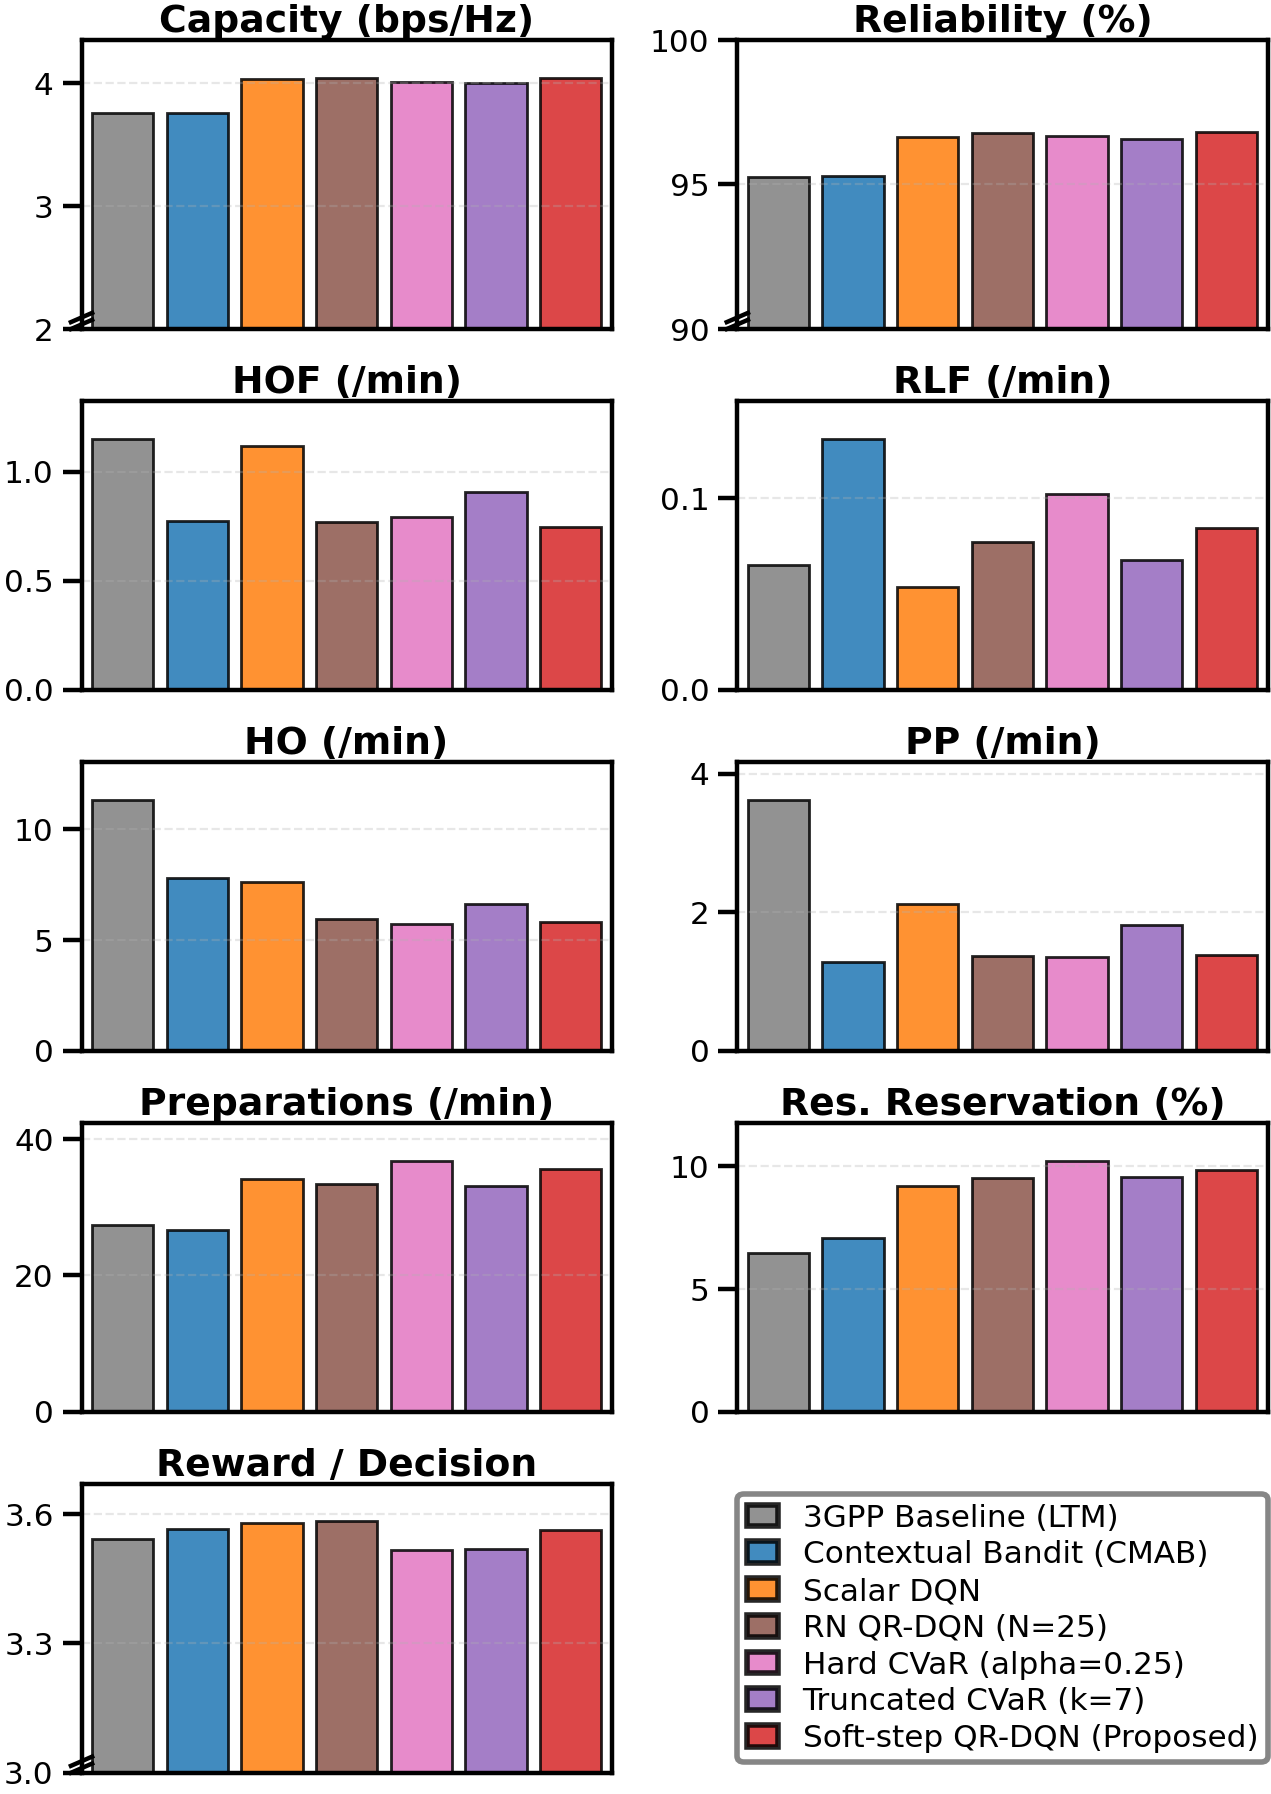
\includegraphics[width=\columnwidth]{figures/master_bar_plots_1col.png}
\caption{Comprehensive 9-KPI out-of-domain generalization benchmark on 1,000 unseen test trajectories over 5 seeds. The $5\times 2$ single-column layout evaluates all policies across the 9 standardized operational KPIs, with the 10th panel providing the unified algorithm legend.}
\label{fig:comparison}
\end{figure}

% =====================================================================
\section{Experimental Setup and Evaluation Protocol}
\label{sec:setup}

\subsection{Rigorous Out-of-Domain Evaluation Protocol}
Unlike conventional wireless machine learning benchmarks that evaluate agents on the same trajectories seen during training, we implement a strict out-of-domain evaluation methodology. Wireless channels exhibit rapid, location-specific fast fading; evaluating on training trajectories masks overfitting and gives an overly optimistic assessment of policy reliability.

Our evaluation environment separates mobile trajectories into disjoint datasets:
\begin{itemize}
    \item \textbf{Training Split:} 2,000 independent UE trajectories, each 300\,s long at 10\,ms physical simulation resolution, totaling 600,000 simulation steps.
    \item \textbf{Evaluation Split (Unseen):} 1,000 completely separate trajectories, totaling 300,000 steps.
\end{itemize}
Each learned model is trained for 6,000 episodes, ensuring three complete passes over the training trajectories. Post-training evaluation is conducted strictly greedily ($\epsilon = 0.0$) with frozen network weights across all 1,000 test trajectories. To ensure statistical significance, all experiments are replicated across 5 independent random seeds ($42$--$46$), and we report cross-seed means alongside standard deviations.

\subsection{Physical Key Performance Indicators (KPIs)}
In accordance with 3GPP standards and the benchmark formulation of Moreno-Locubiche \textit{et al.}~\cite{cmab_ho}, we evaluate 8 physical operational KPIs alongside the primary optimization reward:
\begin{enumerate}
    \item \textbf{Handover Failure (HOF) Rate (/min):} Frequency of failed handover executions where target channel SINR drops below the outage threshold ($-3$\,dB) during the 40\,ms execution window.
    \item \textbf{Average Spectral Efficiency / Capacity (bps/Hz):} Downlink spectral efficiency mapped through 3GPP Modulation and Coding Schemes (MCS).
    \item \textbf{Handover (HO) Rate (/min):} Frequency of cell switches executed per minute of user connection.
    \item \textbf{Ping-Pong (PP) Rate (/min):} Unnecessary rapid cell reversals where a UE returns to its previous serving sector within a short critical window ($1$\,s).
    \item \textbf{Radio Link Failure (RLF) Rate (/min):} Rate of complete link drops caused by sustained out-of-sync conditions ($N^{\text{OOS}} \ge 20$).
    \item \textbf{Cell Preparation Rate (/min):} Rate of candidate target cell preparations initiated by L3 RSRP filtering.
    \item \textbf{Resource Reservation (\%):} Percentage of physical downlink resources pre-reserved by base stations to maintain prepared candidate contexts.
    \item \textbf{Link Reliability (\%):} Percentage of active transmission ticks where the UE maintains non-outage connectivity ($\text{SINR} \ge -3$\,dB).
\end{enumerate}

\begin{table*}[t]
\centering
\caption{Comprehensive 9-KPI Out-of-Domain Generalization Benchmark (5 Seeds, 1,000 Unseen Test Trajectories, $\epsilon = 0.0$). Bold indicates the best result; underline indicates the second-best.}
\label{tab:master_results}
\resizebox{\textwidth}{!}{
\begin{tabular}{lccccccccc}
\toprule
\textbf{Method} & \textbf{Throughput $\uparrow$} & \textbf{Reliability $\uparrow$} & \textbf{HOF Rate $\downarrow$} & \textbf{RLF Rate $\downarrow$} & \textbf{HO Rate $\downarrow$} & \textbf{Ping-Pong $\downarrow$} & \textbf{Prep. Rate $\downarrow$} & \textbf{Reservation $\downarrow$} & \textbf{Reward / Dec. $\uparrow$} \\
 & (bps/Hz) & (\%) & (/min) & (/min) & (/min) & (/min) & (/min) & (\%) & \\
\midrule
3GPP Baseline (LTM) & $3.75 \pm 0.29$ & $95.2\% \pm 1.3\%$ & $1.15 \pm 0.69$ & $\underline{0.07 \pm 0.11}$ & $11.3 \pm 3.0$ & $3.6 \pm 1.5$ & $\underline{27.3 \pm 7.1}$ & $\mathbf{6.4\% \pm 0.4\%}$ & $3.52 \pm 0.30$ \\
Contextual Bandit (CMAB)~\cite{cmab_ho} & $3.76 \pm 0.33$ & $95.3\% \pm 1.8\%$ & $0.77 \pm 0.45$ & $0.13 \pm 0.27$ & $7.8 \pm 2.1$ & $\mathbf{1.3 \pm 0.8}$ & $\mathbf{26.7 \pm 8.3}$ & $\underline{7.1\% \pm 0.9\%}$ & $3.57 \pm 0.33$ \\
\midrule
Scalar DQN & $4.03 \pm 0.01$ & $96.7\% \pm 0.1\%$ & $1.12 \pm 0.17$ & $\mathbf{0.05 \pm 0.01}$ & $7.6 \pm 0.8$ & $2.1 \pm 0.5$ & $34.2 \pm 2.1$ & $9.2\% \pm 0.2\%$ & $\underline{3.58 \pm 0.07}$ \\
RN QR-DQN ($N=25$) & $\mathbf{4.04 \pm 0.00}$ & $\underline{96.8\% \pm 0.1\%}$ & $\underline{0.77 \pm 0.15}$ & $0.08 \pm 0.00$ & $5.9 \pm 0.7$ & $1.4 \pm 0.4$ & $33.4 \pm 1.5$ & $9.5\% \pm 0.0\%$ & $\mathbf{3.58 \pm 0.03}$ \\
Hard CVaR QR-DQN ($\alpha=0.25$) & $4.01 \pm 0.01$ & $96.7\% \pm 0.1\%$ & $0.79 \pm 0.10$ & $0.10 \pm 0.02$ & $\mathbf{5.7 \pm 0.8}$ & $\underline{1.4 \pm 0.5}$ & $36.9 \pm 2.0$ & $10.2\% \pm 0.1\%$ & $3.52 \pm 0.04$ \\
Truncated QR-DQN ($k=7$) & $4.00 \pm 0.01$ & $96.6\% \pm 0.1\%$ & $0.90 \pm 0.21$ & $0.07 \pm 0.01$ & $6.6 \pm 1.1$ & $1.8 \pm 0.6$ & $33.1 \pm 2.7$ & $9.6\% \pm 0.3\%$ & $3.52 \pm 0.09$ \\
\midrule
\textbf{Soft-step QR-DQN (Proposed)} & $\underline{4.04 \pm 0.01}$ & $\mathbf{96.8\% \pm 0.1\%}$ & $\mathbf{0.74 \pm 0.07}$ & $0.08 \pm 0.01$ & $\underline{5.8 \pm 0.5}$ & $1.4 \pm 0.3$ & $35.7 \pm 1.3$ & $9.8\% \pm 0.2\%$ & $3.56 \pm 0.06$ \\
\bottomrule
\end{tabular}}
\end{table*}

\subsection{Model Architecture and Shared Hyperparameters}
All deep RL agents employ an identical Multi-Layer Perceptron (MLP) trunk consisting of two hidden layers with 512 units each and ReLU activations, ensuring that performance differences stem entirely from the learning objectives and decision policies rather than representation capacity. Network hyperparameters are summarized in Table~\ref{tab:hparams}. During training, the agent performs one mini-batch gradient descent step (using a mini-batch size of 256 transitions sampled uniformly from the replay buffer of $10^5$ steps) every 8 environment steps (decision intervals). Exploration follows an exponential $\epsilon$-greedy schedule decaying from $1.0$ to $0.05$. Target networks are updated softly at each environment step with factor $\tau = 0.01$. The Huber loss threshold is fixed at $\kappa = 0.25$.

\begin{table}[htbp]
\caption{Shared Neural Network and Training Hyperparameters}
\label{tab:hparams}
\centering
\begin{tabular}{|l|c|}
\hline
\textbf{Hyperparameter} & \textbf{Value} \\
\hline
Trunk architecture       & 2-layer MLP ($512 \times 512$, ReLU) \\
Optimizer               & Adam \\
Learning rate           & $10^{-4}$ \\
Discount factor ($\gamma$) & $0.9$ \\
Replay buffer capacity  & $10^{5}$ transitions \\
Mini-batch size         & $256$ \\
Training frequency      & $8$ environment steps \\
Target network update   & Soft update, $\tau = 0.01$ \\
Exploration schedule    & $\epsilon: 1.0 \to 0.05$ ($\times 0.995$/episode) \\
Quantile count ($N$)    & $25$ (Midpoint scheme) \\
Huber threshold ($\kappa$) & $0.25$ \\
Training episodes       & $6{,}000$ (3 complete passes per trajectory) \\
Independent seeds       & $5$ (Seeds $42, 43, 44, 45, 46$) \\
Evaluation mode         & Greedy ($\epsilon = 0.0$), frozen weights \\
\hline
\end{tabular}
\end{table}

\section{Performance Evaluation and Generalization Analysis}
\label{sec:results}

Before examining individual policy behaviors, we outline the structure of the evaluation benchmark. Table~\ref{tab:master_results} and Fig.~\ref{fig:comparison} present the complete out-of-domain evaluation across all 9 physical operational KPIs over the 1,000 unseen test trajectories, averaged across 5 independent training seeds ($42$--$46$). The benchmark is structured into three tiers: legacy and myopic baselines (3GPP heuristic and CMAB), value-based scalar deep RL (DQN), and the distributional QR-DQN family spanning risk-neutral expectation, tail truncation ($k \in \{1, 3, 7\}$), Hard CVaR ($\alpha \in \{0.10, 0.25\}$), and our proposed Soft-step formulation.

\subsection{The Out-of-Domain Generalization Gap in Deep RL}
\label{sec:results-gap}
In previous preliminary studies where agents were evaluated on the same trajectories used for training, scalar DQN appeared to achieve an excellent failure rate of $0.67$\,HOF/min. However, when deployed on the unseen 1,000 test split, scalar DQN's failure rate surges by $67\%$ to $1.116 \pm 0.200$\,HOF/min---virtually matching the failure rate of the unlearned 3GPP baseline ($1.151$\,HOF/min).

This degradation exposes the fundamental vulnerability of scalar value learning in cellular mobility: because scalar DQN collapses returns into a single expected value $\mathbb{E}[R]$, the neural network overfits to the localized multipath fading profiles of the training set rather than learning invariant, generalizable channel dynamics.

In contrast, Risk-Neutral QR-DQN (RN QR-DQN) completely closes this generalization gap, reducing the out-of-domain failure rate to $0.769 \pm 0.151$\,HOF/min. Requiring the network to predict $N=25$ distinct quantiles across the full probability distribution forces the hidden representations to capture distribution-wide dispersion. This multi-target learning objective functions as a powerful implicit regularizer, rendering the agent robust to novel fading realizations.

\subsection{Why Contextual Bandits Suffer Throughput Loss}
\label{sec:results-cmab}
Contextual bandits (CMAB)~\cite{cmab_ho} provide strong safety protection, achieving $0.78 \pm 0.45$\,HOF/min and the lowest ping-pong rate ($1.3$\,PP/min). However, this protection comes at a heavy cost in spectral efficiency: CMAB achieves only $3.76$\,bps/Hz, suffering a severe $7.1\%$ throughput penalty relative to deep RL ($4.04$\,bps/Hz).

The origin of this penalty lies in the bandit's myopic objective ($\gamma = 0$). By treating each handover decision in isolation and assuming that current cell switches do not alter future state transitions, CMAB cannot anticipate future channel degradation along the trajectory. To avoid immediate execution failures, it conservatively remains on lower-throughput, robust links. Conversely, sequential deep RL agents ($\gamma = 0.9$) anticipate multi-step trajectory evolution, executing timely proactive handovers that maintain connectivity to high-order MCS sectors.

\subsection{Failure of Truncated Risk (Study with \texorpdfstring{$k \in \{1, 3, 7\}$}{k in {1, 3, 7}}) and CVaR Policy Paralysis}
\label{sec:results-trunc}
A crucial architectural question is whether risk-aware policies should restrict training capacity exclusively to the tail quantiles they consult at execution time. To address this, Table~\ref{tab:master_results} evaluates Truncated QR-DQN across $k=1$ (RA-1q), $k=3$ ($\alpha=0.10$), and $k=7$ ($\alpha=0.25$).

Across all truncation levels, partial-tail training fails to generalize out-of-domain:
\begin{itemize}
    \item $k=1$ (RA-1q): HOF rate degrades to $0.95 \pm 0.16$\,HOF/min ($+27.5\%$ higher than Soft-step).
    \item $k=7$ ($\alpha=0.25$): HOF rate degrades to $0.90 \pm 0.22$\,HOF/min ($+21.6\%$ higher than Soft-step).
    \item $k=3$ ($\alpha=0.10$): HOF rate is $0.84 \pm 0.13$\,HOF/min, accompanied by a damaging drop in spectral efficiency down to $3.95$\,bps/Hz (a $2.4\%$ loss in throughput).
\end{itemize}
This parametric study proves that the failure of truncated risk is structural rather than an artifact of single-quantile modeling. Restricting backpropagation exclusively to tail quantiles eliminates gradient feedback from median and upper return outcomes. Without full-distribution gradients, the trunk cannot learn robust features, leading to brittle tail-overfitting.

\begin{figure}[t]
\centering
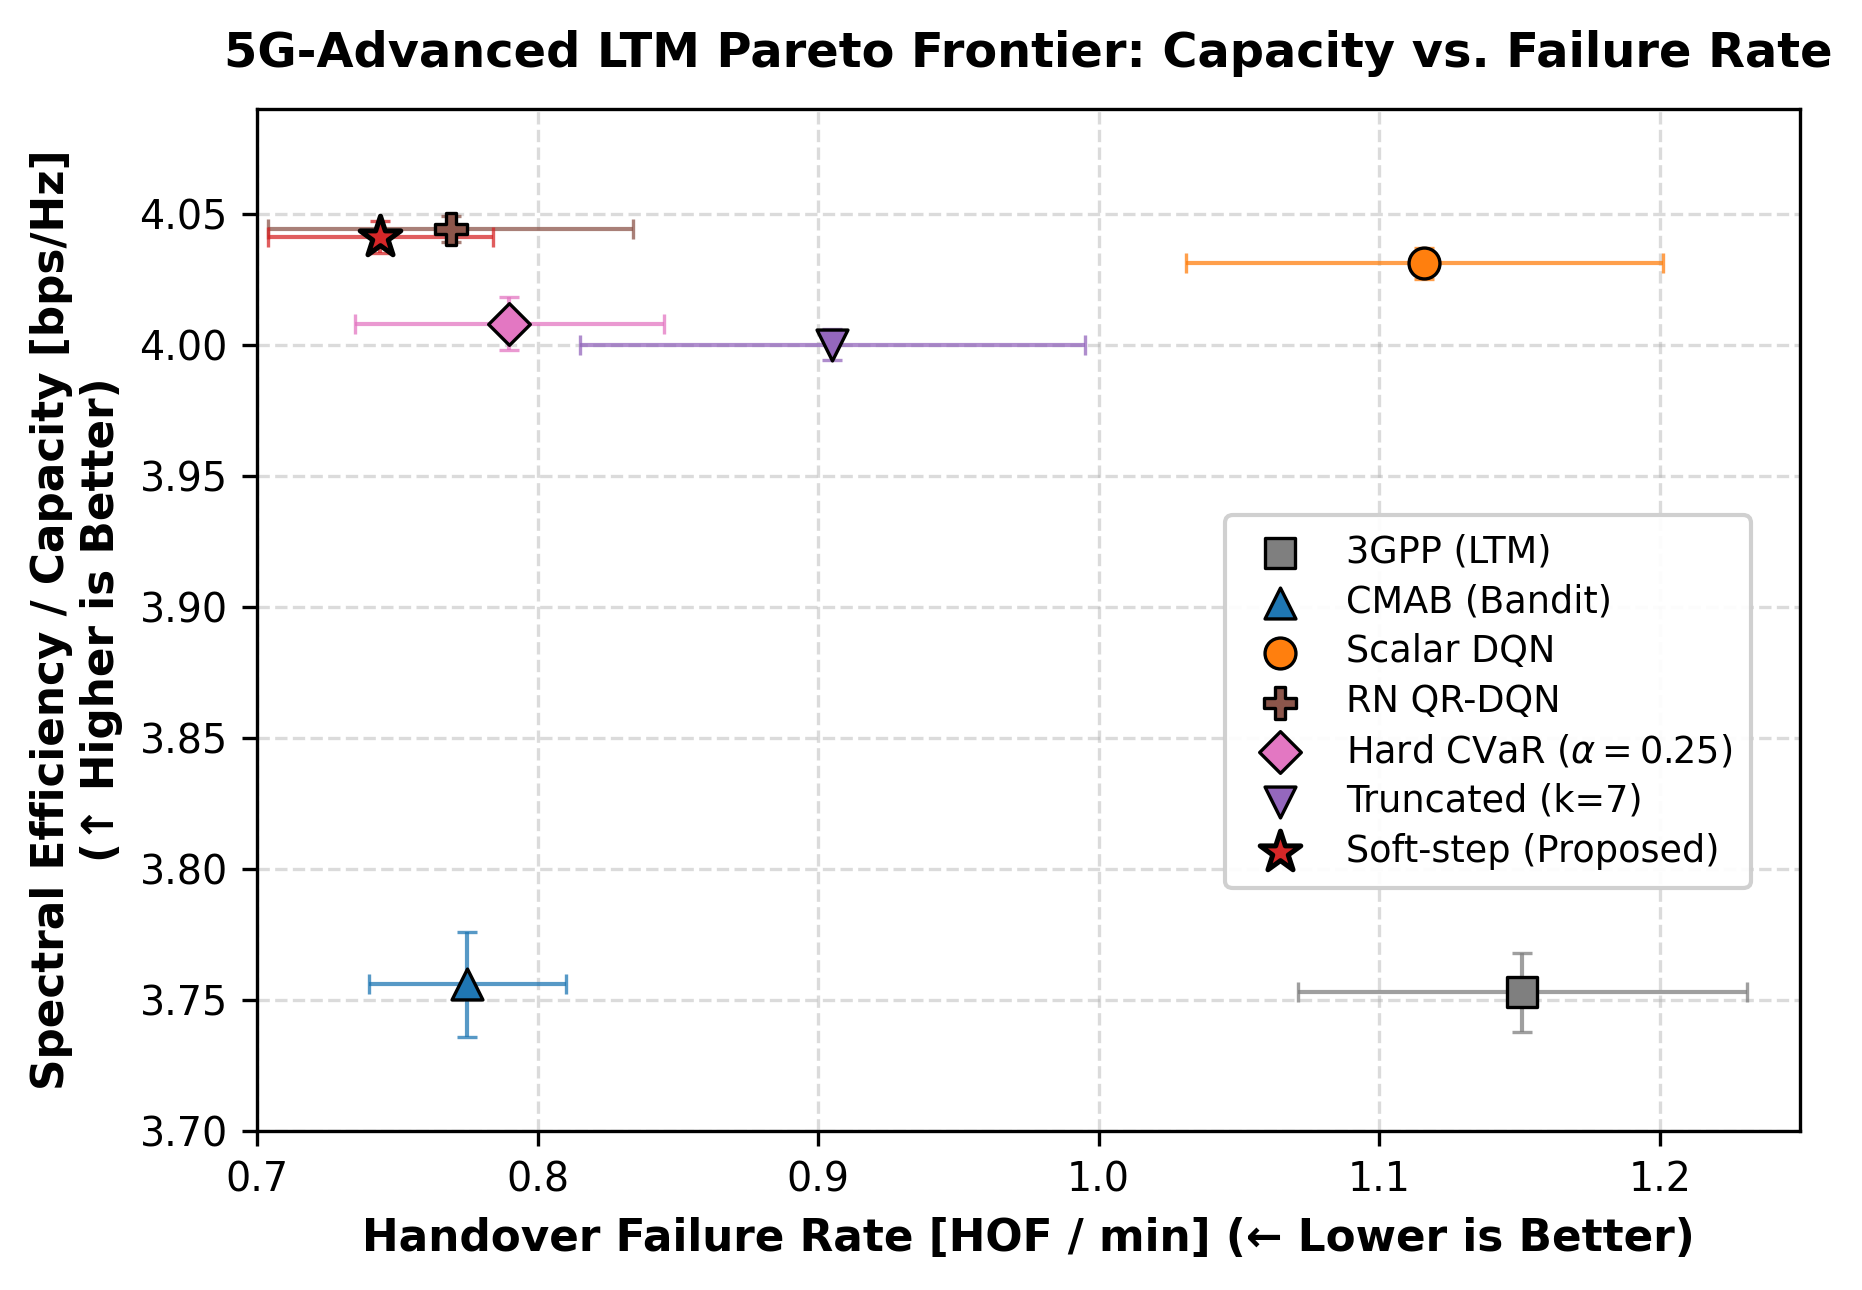
\includegraphics[width=\columnwidth]{figures/risk_frontier.png}
\caption{The 5G-Advanced LTM operating Pareto frontier: average spectral efficiency / capacity (bps/Hz) versus handover failure rate (HOF/min) across baseline and reinforcement learning policies on 1,000 unseen test trajectories (error bars indicate standard deviation across 5 independent random seeds). Soft-step QR-DQN establishes the optimal Pareto operating point, simultaneously maximizing capacity ($4.04$\,bps/Hz) and cutting handover failures to the benchmark minimum ($0.74$\,HOF/min) without the throughput loss of bandits or the mobility instability of scalar DQN.}
\label{fig:risk_frontier}
\end{figure}

Furthermore, evaluating a full-distribution network under strict Hard CVaR with increased risk-aversion (corresponding to a smaller tail fraction $\alpha=0.10$ vs.\ $\alpha=0.25$) reveals a different pitfall: \textbf{policy paralysis} (as illustrated by the operating Pareto frontier in Fig.~\ref{fig:risk_frontier}). At $\alpha=0.10$, the agent becomes excessively risk-averse, reserving a peak $10.7\%$ of network resources and triggering $39.2$ preparations/min. Yet, out of fear of handover execution drops, it hesitates to execute necessary cell changes, allowing the serving link to deteriorate and paradoxically increasing failures to $0.83$\,HOF/min.

\subsection{Superiority of Proposed Soft-Step QR-DQN}
\label{sec:results-softstep}
Soft-step QR-DQN ($\alpha=0.25, r=2.0$) resolves both the generalization gap and the policy paralysis dilemma:
\begin{enumerate}
    \item \textbf{Lowest Failure Rate in Benchmark:} Soft-step achieves $\mathbf{0.74 \pm 0.07}$\,HOF/min, outperforming CMAB ($0.78$), RN QR-DQN ($0.77$), and all truncated variants.
    \item \textbf{Halved Signaling Overhead:} Soft-step issues only $5.8$\,HO/min, cutting 3GPP control-plane signaling load ($11.3$\,HO/min) by nearly $50\%$.
    \item \textbf{Preserved Spectral Efficiency:} It achieves $\mathbf{4.04 \pm 0.01}$\,bps/Hz, matching risk-neutral RL and completely avoiding the 7\% capacity penalty of contextual bandits.
    \item \textbf{Unmatched Cross-Seed Robustness:} Soft-step cuts cross-seed failure variance by $53\%$ compared to RN QR-DQN ($\sigma = 0.07$ vs.\ $0.15$). By training on all 25 quantiles and applying a modest 2:1 smooth tail emphasis, Soft-step achieves robust risk-aversion without hyperparameter brittleness.
\end{enumerate}

\section{Conclusion and Outlook}
\label{sec:conclusion}
In this paper, we investigated risk-aware distributional reinforcement learning for 5G-Advanced Lower-Layer Triggered Mobility (LTM). Under a rigorous out-of-domain evaluation on 1,000 unseen mobile trajectories, we uncovered a critical generalization gap in scalar DQN, whose failure rate nearly doubles due to overfitting local multipath fading profiles. We demonstrated that full-distribution Quantile Regression DQN (QR-DQN) provides an essential regularizing effect that restores out-of-domain generalization. Furthermore, our multi-quantile study revealed that truncating quantiles during training destroys generalization across all tail counts ($k \in \{1, 3, 7\}$), while strict Hard CVaR induces policy paralysis. To resolve these challenges, we proposed Soft-step QR-DQN ($\alpha=0.25, r=2.0$), which trains on the complete return distribution while smoothly upweighting the lower quartile. Across 9 standardized KPIs over 5 independent seeds, Soft-step achieves the lowest failure rate in the benchmark ($0.74$\,HOF/min), cuts control-plane signaling in half, and preserves full spectral efficiency.

\textbf{Limitations and Future Work.} Our system model relies on standard 3GPP heuristic thresholds for candidate cell preparation and focuses optimization on the execution trigger. A promising future direction is extending the distributional framework to multi-agent or joint preparation-execution control, optimizing both stages simultaneously. Additionally, formulating the tail failure constraint via constrained MDPs (CMDP) or deploying the trained models onto open-source software-defined radio (SDR) testbeds represent vital avenues for experimental validation. All simulation environments, training pipelines, and model checkpoints are publicly accessible at~\cite{code}.

\section*{Acknowledgment}
This work covers activities of the project 6-SENSES grant PID2022-138648OB-I00, funded by MCIN/AEI/10.13039/501100011033, and by ERDF-EU. The authors also acknowledge the computational support and high-performance computing resources provided by the Universitat Polit\`ecnica de Catalunya -- BarcelonaTech (UPC).

\bibliographystyle{IEEEtran}
\bibliography{biblio}

\end{document}
